\documentclass{article}
\usepackage{geometry}
\usepackage[utf8]{inputenc}
\usepackage{lmodern}
\usepackage{soul}
\usepackage{babel}
\usepackage{algpseudocode}
\usepackage{fancyhdr}
\usepackage{float}
\usepackage{graphicx}
\usepackage{hyperref}
\usepackage[dvipsnames]{xcolor}
\definecolor{NvidiaGreen}{RGB}{118, 185, 0}
\hypersetup{
  colorlinks   = true,    % Colours links instead of ugly boxes
  urlcolor     = NvidiaGreen,    % Colour for external hyperlinks
  linkcolor    = NvidiaGreen,    % Colour of internal links
  citecolor    = NvidiaGreen      % Colour of citations
}
\usepackage{listings}
\lstset{
   breaklines=true,
   basicstyle=\ttfamily
}
\addto\extrasenglish{%
  \def\chapterautorefname{Chapter}%
  \def\sectionautorefname{Section}%
  \def\subsectionautorefname{Subsection}%
  \def\subsubsectionautorefname{Subsubsection}%
  \def\paragraphautorefname{Paragraph}%
  \def\subparagraphautorefname{Subparagraph}%
}

\title{%
\textsf{%
    \textbf{\textcolor{NvidiaGreen}{N.V.I.D.I.A.\\}}}%
    \large{\textsf{\textbf{``%
    \textcolor{NvidiaGreen}{N}eat %
    \textcolor{NvidiaGreen}{V}ideo %
    \textcolor{NvidiaGreen}{I}nterleaved %
    \textcolor{NvidiaGreen}{D}eblocking %
    \textcolor{NvidiaGreen}{I}nteger %
    \textcolor{NvidiaGreen}{A}lgorithm''}}}%
}
\author{\texttt{GPU Programming} --- $2022$/$2023$}
\date{by \textit{Fulvio Castello} (s$301102$)}

\begin{document}
\maketitle

\section*{Abstract}
In the following, a few basic concepts about video deblocking will be summarized in order to introduce the subject matter while providing a brief technical background on the proposed issue. Then, an extensive overview of the developed program will be presented, explaining the reasoning behind every implementation detail and reflecting on the entire execution flow. The focus will shift on the two alternatives provided by the sequential nature of the \textbf{CPU} in contrast with the parallel architecture of the \textbf{GPU}. After displaying the actual product(s) of the application in question as to prove its practical efficacy, a set of performance comparisons will be drawn whilst making a few considerations regarding both the adopted timing procedure and memory management for data coherence. Finally, the conclusive sections will list the steps needed to run and/or compile and this project, and after that a few personal considerations will be pointed out about the development timeline.

\section{Background}
Video deblocking is a technique used to fix visual artifacts that may appear as a result of bit rate reduction aimed H.$264$ file compression. The most common methods of size reduction make use of the so-called \textit{macroblocks} to approximate the color properties of JPEG pictures. Each frame is masked in such a way that squares of $8\times 8$ pixels become the new computational unit, and all the elements it contains can be shifted toward a common value. In principle, this operation is subject to a given threshold called ``Constant Rate Factor'' (or \textbf{CRF}, in short), that ends up determining the compression ratio and thus the final quality of the end-product. Its values range from $0$ (lossless compression, maximum file size) to $51$ (highly degraded stream, minimum space occupation), with the default being usually set at $23$ for the best trade-off\footnote{\url{https://trac.ffmpeg.org/wiki/Encode/H.264}}.

A deblocking filter is thus applied to an input video stream in order to obtain a cleaner-looking output during runtime, without expanding file size. The calculations required to revert the original approximations are \textbf{dynamic}, in that there is no ``one-size-fits-all'' set of operations that can be universally applied. Execution is \textbf{conditional} by definition, starting from the strength of the effect needed in each individual case. The counterpart of the CRF is in fact represented by the \textit{quantization factor}, which represents the level of correction being applied. Its values range from $1$ to $255$, defaulting to an arbitrary middle-ground of $127$ in this case. Neither of the two aforementioned thresholds gets cached into the video properties or file metadata, and so both conversions are usually achieved optimally by trial-and-error\footnote{\url{https://fotoforensics.com/tutorial.php?tt=estq}}.

There exist many (more or less portable) commercial solutions to tackle this problem, especially after the advent of online streaming services and live broadcasts through the internet, where throughput plays the main role in determining infrastructural limitations. However, arithmetic complexity and computing power requirements are often quite steep --- a simple and efficient alternative has been consequently proposed, providing decent outcomes at a fraction of the effort required by both human and machine\footnote{\url{https://www.researchgate.net/publication/250669132_A_Simple_and_Efficient_Deblocking_Algorithm_for_Low_Bit-Rate_Video_Coding}}.

\section{Implementation}
\textsf{\textbf{N.V.I.D.I.A.}} was created in its entirety by using the CUDA C\texttt{++} programming language, and was thoroughly debugged, tested and profiled on an NVIDIA\textsuperscript{\fontsize{6}{0}\selectfont\textregistered} Jetson Nano\textsuperscript{\fontsize{6}{0}\selectfont ™} Developer Kit\footnote{\url{https://developer.nvidia.com/embedded/jetson-nano-developer-kit}}. The main attributes of this applications are:
\begin{itemize}
    \item \textsf{\textit{Neat}} --- efficient and lightweight computation
    \item \textsf{\textit{Video}} --- computer vision-oriented project
    \item \textsf{\textit{Interleaved}} --- two-pass processing on individual frame channels
    \item \textsf{\textit{Deblocking}} --- aimed at improving visual quality
    \item \textsf{\textit{Integer}} --- comprising integer arithmetic only
    \item \textsf{\textit{Algorithm}} --- dynamic, conditional execution.
\end{itemize}

The program execution starts out with a quite \textbf{fault-tolerant} parsing section: here, the command line arguments are firstly counted and deciphered by means of a \texttt{switch} statement. The only mandatory parameter is the path to the source file, whereas the quantization factor and the output video title can be inferred automatically, but they should figure in the exact order in which they were hereby mentioned (if present). Note that it's still possible to declare just one of them at a time, and their content is gathered in the most flexible way possible. This means that, for instance, any redundant character after the numerical value, or a possible file extension present after the output title, or even useless additional parameters will simply be discarded whilst promptly informing the user. At this point, exceptional program termination will only occur if the inserted values cannot be corrected automatically or in case of file system I/O errors.

After creating the two output video streams with the same exact properties of the source (one used as the destination for the host code and the other for the device), a sequential scan of all frames present in the input takes place. Each of these snapshots will be captured inside a \texttt{cv::Mat} container\footnote{\url{https://docs.opencv.org/4.x/d3/d63/classcv_1_1Mat.html}} provided by the \texttt{OpenCV} library\footnote{\url{https://opencv.org/}}: the corresponding matrix-like structure takes the form of a monolithic $1$-D array of \texttt{unsigned char} elements. These are arranged in such a way that three consecutive bytes represent the value (ranging from $0$ to $255$) of the corresponding color channel. Note that \texttt{OpenCV} automatically saves images in the \textbf{BGR} color space, an equivalent alternative to the well-known RGB format with the red and blue contributions being swapped. Since the proposed algorithm has to work on \textit{luma} and \textit{chroma} values instead, a conversion to \textbf{YCrCb} is first performed\footnote{\url{https://docs.opencv.org/4.7.0/de/d25/imgproc_color_conversions.html}}.

The three newly obtained color components are subsequently split into single-channel \texttt{cv::Mat} containers for convenience. Each of these will be processed individually by both computational units before being merged again into the three-channel output frame. A conversion opposite to before (i.e. \textbf{$\textrm{YCrCb}\rightarrow \textrm{BGR}$}) has to be carried out so that the outcome(s) of the previous computations can be inserted into the corresponding output stream. 

\subsection{Host}
Since the CPU is only capable of sequential execution, the deblocking filter has to work pixel-by-pixel with a \textit{progressive raster scan}, meaning that every frame will be iterated over from position $0$ to position $n=width\cdot height$ (for each of the three channels). The actual calculations are performed in a two-step sequence: first, all the horizontal block edges are corrected, obtaining an intermediate result, to then pass onto the vertical ones inside the same. As a consequence, it's important to underline two key aspects:
\begin{enumerate}
    \item the proposed algorithm acts on each still image in an \textit{incremental} manner, and thus the second pass has to be performed on the transitional frame, causing the two aforementioned steps to be \textbf{interdependent} (and thus not \textit{parallelizable})
    \item despite of the previous point, the order in which these two passes are carried out should be irrelevant. However, given the standard \textbf{progressive scan} approach to display modern-day media, \textit{horizontal} edges were arbitrarily deemed more crucial and are analyzed first (possibly counteracting the intrinsic ``horizontal tearing'' of displays with a fixed frame rate).
\end{enumerate}

The two procedures implementing the actual algorithm of the filter are respectively called \texttt{deblock1h} and \texttt{deblock1v}, both requiring the pointer to the frame data, the quantization scale, the video dimensions and the current pixel identifier. Starting from these parameters, it's possible to derive the coordinates of the considered element inside a $2$-D matrix: this will be called element \texttt{D}, and it will be selected only if it resides on rows/columns that are multiples of $8$ in order to select the boundaries of each macroblock only. Then, the immediately adjacent values on either the $x$ or $y$ axes will follow the same naming convention, obtaining a small array of six units, ranging from \texttt{A} to \texttt{F}. \autoref{macroblock} helps in visualizing the relevant pixels of each frame, considering each of these units as a \texttt{uint8\_t}.

\begin{figure}[!htbp]
  \centering
  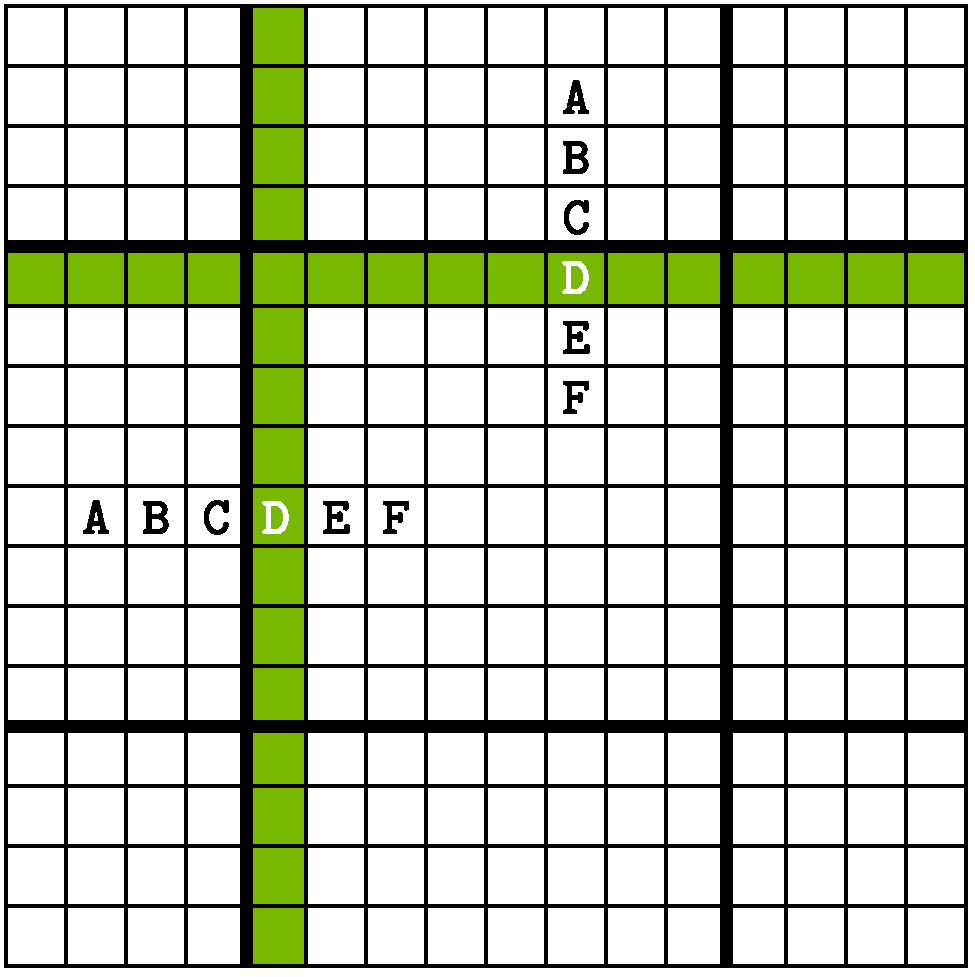
\includegraphics[width=\textwidth]{macroblock.pdf}
  \caption{Structure of a JPEG macroblock used in the proposed algorithm.}
  \label{macroblock}
\end{figure}

At this point, the \textit{adaptive} edge detection can take place, meaning that a \textbf{strong} blocking effect is identified whenever the condition $|B-C|<5\wedge|D-E|<5$ is true, while a \textbf{weak} one is inferred otherwise. In the first case, a larger threshold is taken into account for the subsequent calculations, which in turn target all six positions:
\begin{algorithmic}
    \If{$|C-D|<(2.0\cdot QF)$} 
        \State $x\gets D-C$
        \State $a\gets A+\frac{x}{8}$
        \State $b\gets B+\frac{x}{4}$
        \State $c\gets C+\frac{x}{2}$
        \State $d\gets D-\frac{x}{2}$
        \State $e\gets E-\frac{x}{4}$
        \State $f\gets F-\frac{x}{8}$
    \EndIf
\end{algorithmic}
where lowercase letters represent the output values that have to replace the original ones, and \texttt{QF} is the selected quantization factor. On the other hand, in the complementary situation, only the four inner pixels are modified after evaluating a much stricter condition:
\begin{algorithmic}
    \If{$|C-D|<(0.8\cdot QF)$} 
        \State $x\gets D-C$
        \State $b\gets B+\frac{x}{8}$
        \State $c\gets C+\frac{x}{2}$
        \State $d\gets D-\frac{x}{2}$
        \State $e\gets E-\frac{x}{8}$
    \EndIf
\end{algorithmic}

It's important to note that all calculations are performed on $8$-bit unsigned integer operands, and thus $x$ had to be declared as the next larger signed integer type (i.e. \texttt{int16\_t}) to avoid internal overflows, while the final results are saturated toward $0$ or $255$ as to prevent \textit{clipping}. In all of the above, as much bit-wise arithmetic was used in place of explicit integer algebra as to lighten the computational load of each iteration.

Finally, the entirety of the host code was conceived to be as similar as possible to what would be necessary for the device, and as such many high-level methods and/or properties provided by the \texttt{OpenCV} library were neglected in favor of a more direct approach involving the use of pointers to raw data. This choice is justified by the necessity of creating a fairer and more balanced environment for comparing the two ``competing'' architectures.

\subsection{Device}
The parallel nature of the GPU lends itself very well in computer vision applications such as \textsf{\textbf{N.V.I.D.I.A.}}, particularly thanks to the fact that the underlying matter usually translates to matrix arithmetic. In this case, it was possible to implement the exact same algorithm as described above whilst optimizing its realization:
\begin{enumerate}
    \item the outer \texttt{for} loops were ``unrolled'' into \textit{asynchronous} calls to equivalent CUDA methods by means of three \textbf{streams}, one for each YCrCb channel
    \item the inner \texttt{for} loops were implicitly inferred thanks to the concurrent capabilities of CUDA, in such a way that each kernel gets directly instantiated $n=width\cdot height$ times, covering all pixels \textit{simultaneously}.
\end{enumerate}

Each of the two kernels now work on \texttt{cv::cuda::GpuMat} objects\footnote{\url{https://docs.opencv.org/4.x/d0/d60/classcv_1_1cuda_1_1GpuMat.html}}, which are the device equivalent of the aforementioned \texttt{cv::Mat} containers. Among others, a crucial difference between the two is that the former allocates data on the \texttt{\_\_global\_\_} memory of the GPU in a discontinuous way. This means that consecutive rows of each image might reside in non contiguous addresses, with possible gaps in between. Now the computation of the position inside the data array works in the opposite way compared to before --- gathering the overall index from row and column numbers. Because of the reason just mentioned, the \texttt{step} data member has to be used instead of the total width for this kind of calculation:
\[i=row\cdot \underline{width}+column\Longrightarrow row\cdot\textit{\textbf{step}}+column\]

Each stream is encapsulated in the \texttt{cv::cuda::Stream} wrapper\footnote{\url{https://docs.opencv.org/4.x/d9/df3/classcv_1_1cuda_1_1Stream.html}} and is capable of managing data transfers, event synchronization and kernel execution for each single channel. Regarding the last point, grid and block sizes were chosen as to specify the most regular environment for the CUDA calls, possibly spreading the workload evenly and exploiting the full capabilities of the device. Shared memory ended up remaining unused since each kernel instance has to work on specific pixels only in a conditional fashion, without accumulating any result and only accessing the \texttt{\_\_global\_\_} memory twice (one read and one write) for just a few elements. Constant memory was also out of the question, since there are no \textit{static} features in the proposed algorithm. On the other hand, \textbf{register tiling} proved to be much more useful for the internal calculations of each kernel instance, both in terms of readability and overall bandwidth.

\section{Results}
The filter was tested on two segments of the ``Big Buck Bunny'' animated movie\footnote{\url{https://peach.blender.org/}}, released as an open-source film under \textit{Creative Commons License Attribution 3.0}\footnote{\url{https://creativecommons.org/licenses/by/3.0/}} by the Blender Foundation\footnote{\url{https://www.blender.org/about/foundation/}}. The two files are encoded with different qualities and file extensions, as to prove the flexibility of the \textsf{\textbf{N.V.I.D.I.A.}} application. The outcomes of both the host and the device code are without doubt \textbf{identical}.

The first clip (i.e. \texttt{strong\_sample.mkv}) was used to test the strong filtering portion of the algorithm, after providing the maximum value of $255$ to the QF. A snapshot of a dynamic frame is shown in \autoref{strong0}, to be compared with \autoref{strong1}. The difference is indisputable under all aspects, even if the extremely low starting quality still affects the resulting picture.

\begin{figure}[!htbp]
  \centering
  \includegraphics[width=\textwidth]{strong0.png}
  \caption{Strong blocking effect in \texttt{strong\_sample.mkv}.}
  \label{strong0}
\end{figure}

\begin{figure}[!htbp]
  \centering
  \includegraphics[width=\textwidth]{strong1.png}
  \caption{Strong filtering applied to \texttt{strong\_sample.mkv}.}
  \label{strong1}
\end{figure}

On the other hand, \texttt{weak\_sample.mp4} was processed while leaving the default scale value, and displayed a smoother color gradient in darker areas albeit losing overall picture sharpness. \autoref{weak0} and \autoref{weak1} expose these outcomes by capturing a relevant portion of the picture.

\begin{figure}[!htbp]
  \centering
  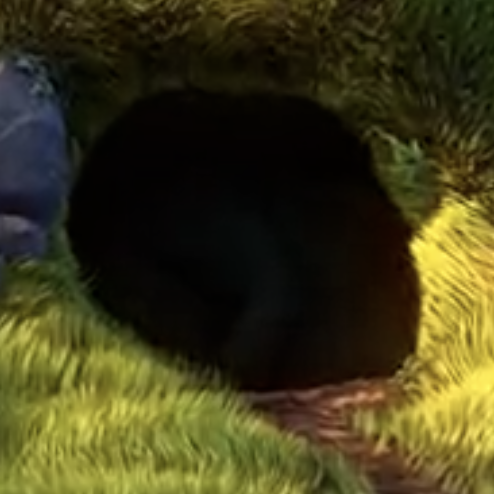
\includegraphics[width=\textwidth]{weak0.png}
  \caption{Weak blocking effect in \texttt{weak\_sample.mp4}.}
  \label{weak0}
\end{figure}

\begin{figure}[!htbp]
  \centering
  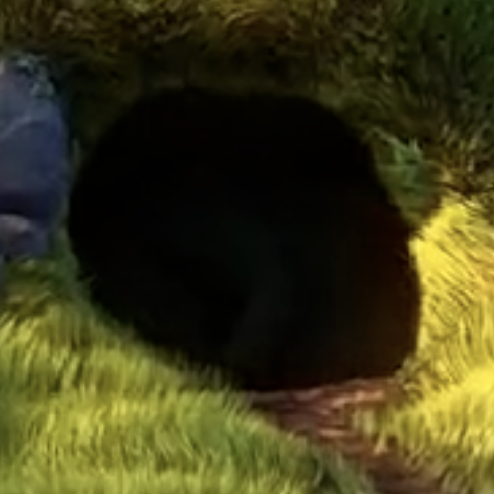
\includegraphics[width=\textwidth]{weak1.png}
  \caption{Weak filtering applied to \texttt{weak\_sample.mp4}.}
  \label{weak1}
\end{figure}

\section{Benchmarks}
Radically different approaches had to be adopted in order to measure the execution time of host and device portions of the program. The \texttt{std::chrono::steady\_clock} high-resolution timer\footnote{\url{https://en.cppreference.com/w/cpp/chrono/steady_clock}} allows to capture the universal time for sequential operations during the flow of the CPU code, in such a way that the duration of each of the two related procedures can easily be obtained by calculating the difference between the starting and the terminating instants. The sum between horizontal and vertical pass then represents the total frame time for the CPU.

Since the GPU runs asynchronous code on three streams, it was necessary to implement a queue of \textbf{events} in order to precisely assess this kind of computation. Three \texttt{cv::cuda::Event} objects\footnote{\url{https://docs.opencv.org/4.x/d5/d38/classcv_1_1cuda_1_1Event.html}} are used in such a way that the duration of every \textit{non-blocking} call can be calculated as the elapsed time between the two adjacent events that surround the corresponding command.

\subsection{Data transfers}
Aside from the execution time of the kernels, all GPU benchmarks also take into account data transfers from host to device and back. Each channel is transferred separately in its own stream, consistently with the corresponding kernel call, thanks to the \texttt{upload} and \texttt{download} methods offered by \texttt{OpenCV}. Since the target platform only features $\mathbf{1}$ \textbf{SM}, this solution is not quite visible in the final benchmarks --- running \textsf{\textbf{N.V.I.D.I.A.}} on more capable hardware could result in a much more noticeable difference.

The concluding snippet of the terminal outputs for both the sample video files are reported in the following. Starting from the strongly blocked stream, the overall improvement resulted in just over $3$X, after processing a total of $125$ frames at $720$p resolution:
\begin{verbatim}
    Video processing complete, please wait...
    - Cumulative CPU time: 20.62 s
       - Horizontal pass: 9.81 s
       - Vertical pass: 10.81 s
    - Cumulative GPU time: 6.72 s
       - Data transfers: 0.62 s
         - HostToDevice: 0.23 s
         - DeviceToHost: 0.39 s
       - Kernel calls: 6.10 s
         - Horizontal pass: 2.15 s
         - Vertical pass: 3.95 s
\end{verbatim}

The second example almost scored $3.5$X over $300$ total frames with same resolution as before. Here, the contribution of data transfers weighs obviously more on the final result because of the longer duration of the video:
\begin{verbatim}
    Video processing complete, please wait...
    - Cumulative CPU time: 48.87 s
       - Horizontal pass: 23.16 s
       - Vertical pass: 25.72 s
    - Cumulative GPU time: 14.49 s
       - Data transfers: 1.42 s
         - HostToDevice: 0.53 s
         - DeviceToHost: 0.89 s
       - Kernel calls: 13.07 s
         - Horizontal pass: 4.72 s
         - Vertical pass: 8.34 s
\end{verbatim}

In order to gather even more precise timing data, the \texttt{nvprof} command was used to test the program in question, and the proportions between all the elapsed periods were comparable. The values were slightly different because of CPU/OS overhead and inherently approximate synchronization between events during the observable runtime of the application.

\section{Instruction manual}
This project was compiled on the official Ubuntu distribution provided by NVIDIA for the target platform in question\footnote{\url{https://developer.nvidia.com/embedded/learn/get-started-jetson-nano-devkit\#write}}. It can be run by opening a terminal inside the same directory of the \texttt{deblock} executable and passing the following command:
\begin{center}
    \texttt{./deblock path/to/file [QF] [output\_title]}
\end{center}
where only the first argument is mandatory and redundant ones will simply be discarded. The program will begin to print out the benchmarks of each single frame, before reporting a final summary of the whole runtime. Any explicit note, warning or error is printed out for the end user, while other kinds of internal exceptions might be thrown by the \texttt{OpenCV} library and its included packages before aborting the execution.

The output files will be located inside two newly created folders called ``cpu'' and ``gpu'' for the homonymous architectures. Note that the original stream will be stripped of its audio track, since that is currently not natively supported by the libraries this application relies upon.

\subsection{Compilation}
In order to compile this project on any other platform of choice, it's possible to use the given \textit{Makefile}, which is a modified version of the one provided inside the demo examples found in every CUDA installation. The \texttt{make} command can be used to generate the \texttt{deblock} executable, while \texttt{make clean} completely removes the application from the file system.

Two major dependencies are required in order to perform this manual step:
\begin{enumerate}
    \item the system must have a CUDA-capable NVIDIA graphics card with the CUDA framework correctly installed and configured\footnote{\url{https://developer.nvidia.com/cuda-downloads}}
    \item the \texttt{OpenCV} library must be installed with the following flags (amongst others, if needed)\footnote{\url{https://docs.opencv.org/4.x/d0/d3d/tutorial_general_install.html}}:
        \begin{verbatim}
        -D CMAKE_BUILD_TYPE=RELEASE
        -D WITH_CUDA=ON
        -D WITH_CUDNN=ON
        -D WITH_CUBLAS=ON
        -D WITH_TBB=ON
        -D OPENCV_DNN_CUDA=ON
        -D OPENCV_ENABLE_NONFREE=ON
        -D OPENCV_GENERATE_PKGCONFIG=ON
        -D CUDA_ARCH_BIN=??
        \end{verbatim}
    where the compute capability has to be known for the target architecture\footnote{\url{https://developer.nvidia.com/cuda-gpus}}.
\end{enumerate}

If both installations are able complete successfully, any recent device should be able to comfortably run this lightweight application in a matter of minutes or even seconds, depending on the total number of frames.

\section{Conclusion}
This project revolved around implementing a given algorithm in a familiar programming language, and then optimizing its execution by exploiting the capabilities of the CUDA framework. While the timing performance of this program was always the main focus of the development timeline, many of peculiar aspects about computer vision and a lot of background knowledge had to be acquired in advance, representing the real value of this assignment. Since the latter was an individual work, a multitude of challenges continuously emerged and took a considerable amount of effort to be solved without the possibility of discussing and reasoning with a possible team mate. On the other hand, every decision was swiftly taken with no confrontation needed, and a single mind was easily able to manage the evolution of the project at any time.

Many improvements could probably be applied to this product, the most evident ones being the introduction of audio support as well and the alteration of the deblocking algorithm in order to make the two passes independent from each other, maybe even merging them into one single step.

\end{document}
